\chapter{Complex Rayleigh Quotient Iteration}
In this chapter we introduce \emph{Complex Rayleigh Quotient
  Iteration} (CRQI\footnote{We abbreviate the classic Rayleigh
  Quotient Iteration that was discussed in the previous chapter by
  \emph{RQI} or \emph{classic RQI} and the method introduced in this
  chapter by \emph{CRQI}.}). This is a novel shift-and-invert
algorithm similar to classic RQI. Numerical experiments suggest that
this new method overcomes some of the disadvantages of classic RQI.
In particular, it seems to perform well in cases when there are
eigenvalues very close to the target eigenvalue but a good
approximation of the eigenvector is known.

\section{Motivation}
As was the case in the previous chapters we fix a real symmetric
matrix $\mat{A} \in \R^{n \times n}$. Recall that since the
eigenvectors $\vec{v}_1, \dotsc, \vec{v}_n$ of $\mat{A}$ form an
orthonormal basis of $\R^n$ we can write every $\vec{u} \in \R^n$ as
\[
  \vec{u} = \sum_{i=1}^n \alpha_i \vec{v}_i
\]
for certain $\alpha_1, \dotsc, \alpha_n \in \R$. Suppose now, that
$\vec{u}$ is a good approximation for one of the eigenvectors, say for
$\vec{v}_k$. Then
\[
  \alpha_k \approx 1 \qquad \text{and} \qquad \alpha_j \approx 0 \
  \text{ for } \ j \neq k \,.
\]
Due to the pairwise orthogonality of the eigenvectors this implies
\begin{equation}
  \label{eq:guess_orthogonal}
  \vec{u}^\tp \vec{v}_j \approx
  \begin{cases} 
    1 & \text{ if } j = k \,, \\
    0 & \text{ if } j \neq k \,.
  \end{cases}
\end{equation}
As already mentioned previously, when using classic RQI even good
approximations of eigenvectors can lead to convergence to the wrong
eigenpair when the gap between the target eigenvalue and eigenvalues
nearby is very small. We will illustrate this behaviour in different
examples in the next section. There, we will see that the reason for
this seems to be that classic RQI does not ``incorporate'' the
information in the initial vector. The main purpose of complex RQI is
to fix this, \ie to alter classic RQI in such a way that for
sufficiently good approximations of eigenvectors convergence to this
very eigenvector is guaranteed.

To that end, the linear system that is solved at each step in RQI is
perturbed in such a way that the wanted eigenvalue gets
``isolated''. Of course this perturbed linear system will lead to
wrong solutions and so we will decrease this perturbation successively
until we arrive at the unperturbed problem. \todo{Explain a bit more}

We make use of the fact that all eigenvalues of $\mat{A}$ are real and
perturb the matrix in such a way that the eigenvalues are ``raised''
into the complex plane. Of course, we do not want to raise them all
equally but rather in such a way that the Euclidean distance between
the target eigenvalue and the other eigenvalue is increased. This is
done by incorporating the approximation $\vec{u}$ of the target
eigenvector $\vec{v}_k$ into the perturbed matrix. Let
\begin{equation}
  \label{eq:a:tilde}
  \tilde{\mat{A}} \coloneqq \mat{A} - \gamma i(\mat{I} - \vec{u} \vec{u}^\tp)\,,
\end{equation}
where $\gamma > 0$ is positive real number and $i$ denotes the
imaginary unit. Note that the matrix $\mat{I} - \vec{u} \vec{u}^\tp$
defines the orthogonal projection onto the span of $\vec{u}$.
Therefore, a vector $\vec{x}$ that is almost parallel to $\vec{u}$
will barely see the imaginary part
$\gamma i (\mat{I} - \vec{u} \vec{u}^\tp)$ when multiplied with
$\tilde{\mat{A}}$ and so
$\tilde{\mat{A}} \vec{x} \approx \mat{A}\vec{x}$. If, however, the
vector $\vec{x}$ is almost perpendicular to $\vec{u}$ we have
\begin{equation}
  \label{eq:a:tilde:multorth}
  \tilde{\mat{A}} \vec{x} = \mat{A}\vec{x} - \gamma i \vec{x} - \vec{u}
  \underbrace{\vec{u}^\tp \vec{x}}_{\approx 0} \approx (\mat{A} - \gamma i \mat{I})\vec{x}\,.
\end{equation}
Since $\vec{u}$ approximates $\vec{v}_k$, the orthogonal complement of
the span of $\vec{u}$ approximates the orthogonal complement of the
span of $\vec{v}_k$. Note that the latter is the subspace spanned by
the remaining eigenvectors. Therefore, we expect that the eigenvectors
of $\tilde{\mat{A}}$ are similar to those of $\mat{A}$ and that the
eigenvalues corresponding to eigenvectors $\vec{v}_j$, $j \neq k$ to
approximately be $\lambda_j - \gamma i$ due
to~\eqref{eq:a:tilde:multorth}. The eigenvalue corresponding to
$\vec{v}_k$ would then be approximately equal to $\lambda_k$ since
$\tilde{\mat{A}}\vec{v}_k \approx \mat{A}\vec{v}_k = \lambda_k
\vec{v}_k$.

To make this intuition more quantitative, we first need the following
result where we replace $\vec{u}$ by the exact target eigenvector
$\vec{v}_k$. The proofs for the following results can be found in
Appendix~\ref{appendix:proofs}.
\begin{lemma}%
  \label{lem:eigs:atilde0}
  The matrix
  \begin{equation}
    \label{eq:a:tilde0}
    \tilde{\mat{A}}_{(0)} \coloneqq \mat{A} - \gamma i(\mat{I}- \vec{v}_k \vec{v}_k^\tp)
  \end{equation}
  has the same eigenvectors as $\mat{A}$ with corresponding
  eigenvalues
  $\lambda_j(\tilde{\mat{A}}_{(0)}) = \lambda_j(\mat{A}) - \gamma i$
  for $j \neq k$ and
  $\lambda_k(\tilde{\mat{A}}_{(0)}) = \lambda_k(\mat{A})$.
\end{lemma}

To derive estimations for the eigenvalues of $\tilde{\mat{A}}$, we
decompose it into the sum
$\tilde{\mat{A}} = \tilde{\mat{A}}_{(0)} + \tilde{\mat{A}}_{(1)}$,
where $\tilde{\mat{A}}_{(0)}$ is defined in~\eqref{eq:a:tilde0} and
$\tilde{\mat{A}}_{(1)}$ is given by
\begin{equation}
  \label{eq:a:tilde1}
  \tilde{\mat{A}}_{(1)} \coloneqq \gamma i ( \vec{u} \vec{u}^\tp - \vec{v}_k\vec{v}_k^\tp)\,.
\end{equation}

Since $\vec{u}$ approximates $\vec{v}_k$ we expect the effect on the
\todo{Replace effect} eigenvalues of $\tilde{\mat{A}}_{(0)}$ due to
the perturbation $\tilde{\mat{A}}_{(1)}$ to be small. The following
lemma answers how ``big'' this perturbation is.

% As long as both $\gamma$ and the angle between the vector $\vec{u}$
% and the wanted eigenvector are sufficiently small this is indeed the
% case as the following lemma shows.

\begin{lemma}
  Let $\tilde{\mat{A}}_{(1)}$ be the matrix defined in
  Equation~\eqref{eq:a:tilde1}. Then
  \begin{equation}
    \label{eq:a:tilde1:norm}
    \norm{\tilde{\mat{A}}_{(1)}} = \gamma \sqrt{1 - {\langle \vec{u}, \vec{v}_k \rangle}^2}\,.
  \end{equation}
\end{lemma}
For good approximations $\vec{u}$ we have
${\langle \vec{u}, \vec{v}_k \rangle}^2 \approx 1$ and thus, if
$\gamma$ is sufficiently small, $\norm*{\tilde{\mat{A}}_{(1)}} \ll 1$.
We can now estimate the eigenvalues of $\tilde{\mat{A}}$.

\begin{proposition}
  The eigenvalues of $\tilde{\mat{A}}$ satisfy
  \begin{equation}
    \label{eq:a:tilde:eigvalbound}
    \lambda_j(\tilde{\mat{A}}) =
    \lambda_j(\mat{A}) + \gamma i\left({\langle \vec{v}_j, \vec{u} \rangle}^2 - 1\right)
    + \mathcal{O}\left(
      \norm{\tilde{\mat{A}}_{(1)}}^2
    \right)\,,
  \end{equation}
\end{proposition}

As mentioned above the proof can be found in the Appendix. It uses
classic results from analytic perturbation theory. To understand why
this matches our intuitive arguments from above we consider the middle
part of~\eqref{eq:a:tilde:eigvalbound}. For $j \neq k$ the scalar
product is approximately zero and thus, if we ignore the last term of
the sum (which is small according to the previous lemma), we get
\begin{equation*}
  \lambda_j(\tilde{\mat{A}}) \approx \lambda_j(\mat{A}) - \gamma i\,.
\end{equation*}
For $j = k$ the middle part is negligible due to the scalar product
being approximately one and so
$\lambda_k(\tilde{\mat{A}}) \approx \lambda_k(\mat{A})$. In summary,
the eigenvalue corresponding to the wanted eigenvector stays near the
real line whereas the remaining eigenvalues are raised into the lower
complex half-plane.

If we would use this matrix in RQI, the results would of course not be
the target eigenpair but an eigenpair of $\tilde{\mat{A}}$. Thus,
instead of keeping this matrix fixed, we replace the vector $\vec{u}$
by the current iterate $\vec{x}^{(k)}$ and the scalar $\gamma$ by a
sequence $\gamma^{(k)}$ that converges to zero. Ideally, in the
beginning of the iteration $\gamma^{(k)}$ should be sufficiently large
such that the target eigenvalue is properly isolated. As the the
iterates get closer to the target eigenpair, $\gamma^{(k)}$ should
decrease such that in the end $\tilde{\mat{A}} \approx \mat{A}$. A
possibly choice that comes to mind is the norm of the current residual
$\vec{r}^{(k)}$ or related quantities such as the square of the
residual norm. How the choice of this shift influences the convergence
behaviour is discussed in the next first example of
Section~\ref{sec:crqi:experiments}.  Obviously, we cannot expect this
method to attain local cubic convergence. The matrix $\tilde{\mat{A}}$
is neither symmetric nor Hermitian but of complex symmetric type. As
we will see shortly, however, if good approximations of the wanted
eigenvector are used for the initial vector the method often requires
merely three or four additional steps compared to classic RQI.

Another problem seems to be that if $\mat{A}$ is sparse,
$\tilde{\mat{A}}$ will in general not be sparse. In fact, the
perturbed matrix will quite possibly posses only few, if any, zero
entries. This seemingly severe disadvantage will shortly be resolved.
We will see that it is in fact not necessary to perturb the matrix by
$\gamma i(\mat{I} - \vec{u}\vec{u}^\tp)$. It suffices to subtract from
$\mat{A}$ the diagonal matrix $\gamma i \mat{I}$ and the method
presented above was merely for motivational purposes. The resulting
matrix is still complex symmetric but now only the diagonal entries
are altered and sparsity is preserved.

\section{Implementation}

Although we will soon slightly change the matrix $\tilde{\mat{A}}$
defined in~\eqref{eq:a:tilde} again, we summarise the discussion up to
this point in Algorithm~\ref{alg:crqi:proj}.\footnote{By
  $\Re(\vec{x})$ we denote the real part of the complex vector
  $\vec{x}$.}

\begin{algorithm}[htpb]
  \DontPrintSemicolon%
  \KwData{Nonzero initial vector $\vec{x}^{(0)}$ with $\norm*{\vec{x}^{(0)}} = 1$}
  \Begin{
    $\mu^{(0)} \gets {(\vec{x}^{(0)})}^\herm \mat{A} \vec{x}^{(0)}$\;
    $r^{(0)} \gets \norm*{(\mat{A} - \mu^{(0)}\mat{I}) \vec{x}^{(0)}}$\;
    $\gamma^{(0)} \gets r^{(0)}$\;
    \For{$k = 1,2,\dotsc$ until convergence}{
      $\tilde{\mat{A}} \gets \mat{A} - \gamma^{(k)}i(\mat{I} - \vec{x}^{(k)} {(\vec{x}^{(k)})}^\herm)$\;
      Solve $( \tilde{\mat{A}} - \mu^{(k)}\mat{I})\tilde{\vec{x}}^{(k+1)} = \vec{x}^{(k)}$\;
      $\vec{x}^{(k+1)} \gets \tilde{\vec{x}}^{(k+1)} / \norm*{\tilde{\vec{x}}^{(k+1)}}$\;
      $\mu^{(k+1)} \gets {(\vec{x}^{(k+1)})}^\herm \mat{A} \vec{x}^{(k+1)}$\;
      $r^{(k+1)} \gets \norm*{(\mat{A} - \mu^{(k+1)}\mat{I}) \vec{x}^{(k+1)}}$\;
      $\gamma^{(k+1)} \gets r^{(k+1)}$\;
    }
    $\vec{x} \gets \Re({\vec{x}^{(k+1)}})$\;
    $\vec{x} \gets \vec{x} / \norm*{\vec{x}}$
  }
  \caption{Complex Rayleigh Quotient Iteration, First Version}\label{alg:crqi:proj}
\end{algorithm}
\todo{Sign of shift in Algo step should be +?}

Strictly speaking, this algorithm is not a Rayleigh Quotient Iteration
as the matrix changes at each step. Obviously, the method is strongly
linked to RQI so we still refer to it as Complex Rayleigh Quotient
Iteration. As mentioned above, this is not the final version as we
wish to present it. The following lemma allows for a small
simplification of the algorithm.

\begin{lemma}
  Let $\mat{A} \in \R^{n \times n}$ be a non-singular real symmetric
  matrix. Let $\vec{u} \in \C^n$ be a unit vector. We define the
  matrices
  \begin{equation}
    \label{eq:rayleigh_quotient_complex}
    \mat{B} \coloneqq \mat{A} - (\sigma - \gamma i) \mat{I}
  \end{equation}
  and
  \begin{equation}
    \label{eq:rayleigh_quotient_proj}
    \mat{C} \coloneqq { \mat{A} - \sigma \mat{I} + \gamma i( \mat{I} - \vec{u} \vec{u}^\herm)}\,,
  \end{equation}
  where $i$ is the imaginary unit and $\sigma, \gamma > 0$ are
  positive real numbers such that $\sigma$ is not an eigenvalue of
  $\mat{A}$. Then
  \begin{equation}
    \label{eq:rq_equal}
    \rq_{\mat{A}}(\mat{B}^{-1} \vec{u}) = \rq_{\mat{A}}(\mat{C}^{-1} \vec{u} ) \,.
  \end{equation}
\end{lemma}
\begin{proof}
  Without loss of generality, we can assume $\sigma = 0$. Otherwise,
  set $\tilde{\mat{A}} = \mat{A} - \sigma \mat{I}$ and use this matrix
  instead of $\mat{A}$ ($\tilde{\mat{A}}$ is obviously still real and
  symmetric and invertible since $\sigma$ is not an eigenvalue of
  $\mat{A}$). First, observe that
  $\mat{C} = \mat{B} - \gamma i \vec{u}\vec{u}^\herm$. Using the
  Sherman-Morrison formula~\cite{hager1989update} and letting
  $\alpha \coloneqq 1 - \gamma i \vec{u}^\herm \mat{B}^{-1} \vec{u} \,
  \in \C$ we obtain
  \begin{align*}
    \mat{C}^{-1} \vec{u} &= {\left( \mat{B} - \gamma i \vec{u} \vec{u}^\herm \right)}^{-1} \vec{u} \\
                         &= \left(
                           \mat{B}^{-1} + \alpha^{-1} \mat{B}^{-1} \vec{u} \gamma i \vec{u}^\herm \mat{B}^{-1}
                           \right) \vec{u} \\
                         &= \mat{B}^{-1} \vec{u} + \mat{B}^{-1} \vec{u} \underbrace{\alpha^{-1} \gamma i \vec{u}^\herm \mat{B}^{-1} \vec{u} }_{ \in \C} \\
                         &= \mat{B}^{-1} \vec{u} ( 1 + \alpha^{-1} \gamma i \vec{u}^\herm \mat{B}^{-1} \vec{u}) \,.    
  \end{align*}
  Thus, the vector $\mat{C}^{-1} \vec{u}$ is a scalar multiple of
  $\mat{B}^{-1} \vec{u}$ and the result follows from
  Lemma~\ref{lem:rq:properties} (i) (the Homogeneity of the Rayleigh
  Quotient).
\end{proof}
\todo{Where is the non-singularity needed?}

Immediately, the following result follows.

\begin{corollary}
  Algorithm~\ref{alg:crqi:proj} produces the same results when
  $\tilde{\mat{A}}$ is replaced with
  $\hat{\mat{A}} = \mat{A} + \gamma i \mat{I}$.
\end{corollary}
\begin{proof}
  
\end{proof}
This result allows for a simplification of the algorithm. We combine
the real shift $\mu^{(k)}$ and the imaginary shift $i \gamma^{(k)}$
into a new shift $\sigma^{(k)} \coloneqq \mu^{(k)} - i \gamma^{(k)}$
and solve the system
\begin{equation*}
  (\mat{A} - \sigma^{(k)} \mat{I}) \vec{x}^{(k+1)} = \vec{x}^{(k)}
\end{equation*}
for $\vec{x}^{(k+1)}$ at each step.



\section{Numerical Experiments}\label{sec:crqi:experiments}
In this section we discuss different numerical examples to better
understand the behaviour of CRQI. Throughout the section we will
always compare the method to classic RQI. All experiments were
executed in Matlab 9\todo{Cite matlab}. The criterion for convergence
was
$\norm*{\vec{r}^{(k)}} = \norm*{\mat{A}\vec{x}^{(k)} - \mu^{(k)}
  \vec{x}^{(k)}} < 10^{-8}$. The source codes for both classic and
complex RQI can be found in the Appendix. The methods are defined
slightly differently from the Algorithms given above. They both allow
to explicitly set the initial shifts $\mu^{(0)}$ and $\gamma^{(0)}$ to
specific values whereas in Algorithm~\ref{alg:rqi} and
Algorithm~\ref{alg:crqi:proj} the initial shifts are always
initialised as the Rayleigh Quotient of the initial vector and the
initial residual, respectively. In most of the examples below the
matrix $\mat{A}$ was a randomly generated sparse symmetric
$200 \times 200$ matrix. To simulate that a good approximation of the
initial vector is available we computed the full set of eigenvectors
collected as columns of the matrix $\mat{V}$. Next, a weight vector
$\vec{w}$ of uniformly distributed numbers between $0$ and $1$ is
created. One of the components is set to a higher value than the
others, \eg $w_{50} = 10$ (in most examples the index of the component
was also chosen randomly). The initial vector is then set to a
weighted linear combination of the eigenvectors, \ie
$\vec{x}^{(0)} = \beta \mat{V} \vec{w}$, where $\beta$ has to be
chosen such that $\vec{x}^{(0)}$ is normalised. Now, $\vec{x}^{(0)}$
is a vector with a strong component in the direction of the target
eigenvector and random (smaller) contributions in the directions of
the other eigenvectors.

The first example demonstrates the influence of the imaginary shift
$\gamma^{(k)} i$ on the convergence speed. We started by running two
versions of CRQI. The first uses
$\gamma^{(k)} = \norm*{\vec{r}^{(k)}}$, the second uses the square of
the residual norm. A plot of the residuals against the iteration
number of both these approaches together with the results using
classic RQI\footnote{Classic RQI is merely included for speed
  comparison. Since the eigenvalues of the test problem are closely
  spaced, in almost all of the examples classic RQI failed to converge
  to the right eigenvalue.} and a third approach described shortly is
given in Figure~\ref{fig:residuals}.

\begin{figure}[htpb]
  \centering
  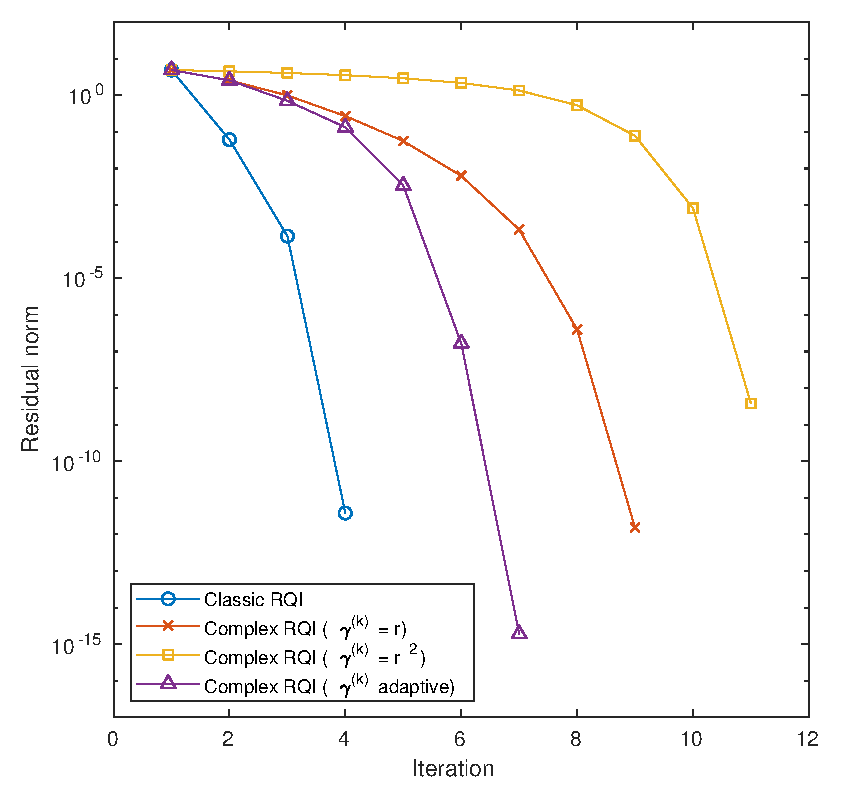
\includegraphics[width=0.7\textwidth]{Figures/crqi_residuals}
  \caption[Residuals for different choices of $\gamma^{(k)}$.]{Plot of
    residuals of Classic RQI, Complex RQI with
    $\gamma^{(k)} = \norm*{\vec{r}^{(k)}}$, Complex RQI with
    $\gamma^{(k)} = \norm*{\vec{r}^{(k)}}^2$ and Complex RQI with the
    imaginary shift chosen adaptively (see text). The last variantt
    seems to combine the adavantages of the second and third
    alternatives.}%
  \label{fig:residuals}
\end{figure}

We observe that in the initial phase of the iteration, the second
variant seems to be slower than the first. Altough it is not clearly
observable in the figure below, other examples suggested that during
the final steps of the iterations the second version was faster than
the first. Consequently, by combining both approaches and thus
changing the shift adaptively we expect faster convergence. The
results are also plotted in Figure~\ref{fig:residuals} and are in
accordance with the expectation. In this particular case, the shift
was changed adaptively according to
\begin{equation*}
  \gamma =
  \begin{cases}
    \norm*{\vec{r}} & \text{ if } \norm*{\vec{r}} \ge 1\,, \\
    \norm*{\vec{r}}^2 & \text{ if } \norm*{\vec{r}} < 1\,,
  \end{cases}
\end{equation*}
where we dropped the superscripts from $\gamma = \gamma^{(k)}$ and
$\vec{r} = \vec{r}^{(k)}$. In the following, when we speak of CRQI we
mean CRQI performed with this adaptive choice of imaginary shifts.

Running the same experiment but increasing the component of the
initial vector in the direction of the target eigenvector it showed
that the number of additional steps required by CRQI diminshed. For
eigenvectors that were very close to the target sometimes both classic
RQI and complex RQI finished within the same number of iterations and
while CRQI generally produced the correct eigenpair, classic RQI
usually failed to do so.

\begin{figure}[htpb]
  \centering
  \begin{subfigure}[b]{0.475\textwidth}%
    \centering
    \includegraphics[width=\textwidth]{Figures/crqi_varyingshift__initvec_small_direction_70deg_negative}%
    \caption{{\small Small component in target direction, negative
        eigenvalue}}%
    \label{fig:varying shift small negative}
  \end{subfigure}%
  \hfill
  \begin{subfigure}[b]{0.475\textwidth}%
    \centering
    \includegraphics[width=\textwidth]{Figures/crqi_varyingshift__initvec_small_direction_70deg}%
    \caption{{\small Small component in target direction, positive
        eigenvalue}}%
    \label{fig:varying shift small positive}
  \end{subfigure}
  \vskip\baselineskip
  \begin{subfigure}[t]{0.475\textwidth}%
    \centering
    \includegraphics[width=\textwidth]{Figures/crqi_varyingshift__initvec_suffctl_big}%
    \caption{{\small Sufficiently big component in target direction}}%
    \label{fig:varying shift big}
  \end{subfigure}
  \hfill
  \begin{subfigure}[t]{0.475\textwidth}%
    \centering
    \includegraphics[width=\textwidth]{Figures/crqi_varyingshift__initvec_random}%
    \caption{{\small Random initial vector}}%
    \label{fig:varying shift random}
  \end{subfigure}
  \caption[RQI and CRQI wiith varying initial shifts]{Plot of initial
    real shift against the computed eigenvalue using classic RQI and
    CRQI. The dotted area encloses the initial shifts that lie in the
    spectrum of $\mat{A}$. In the first two examples the initial
    vector had only a small component in the direction of the target
    eigenvector. }
  \label{fig:vary shift}
\end{figure}

Further investigation revealed that the behaviour as in
Figure~\ref{fig:varying shift small positive} and
Figure~\ref{fig:varying shift small negative}
%%% Local Variables: 
%%% mode: latex
%%% TeX-master: "../../main"
%%% End:





% used as an initial guess in the classic Rayleigh Quotient Iteration.
% We can, however, use~\eqref{eq:guess_orthogonal} to shift the
% eigenvalues in such a way that the distance between the target
% eigenvalue and adjacent eigenvalues is increased. This fact is then
% used to alter the linear system that is solved at each step in the
% Rayleigh Quotient Iteration, increasing the chance that the method
% will converge to the right eigenpair.

% We first observe that given a vector $\vec{x} \in \R^n$, the
% projection of $\vec{x} \in \R^n$ onto the span of a unit vector
% $\vec{u}$ is
% \[
%   (\vec{u}^\tp \vec{x})\vec{u} = \vec{u}(\vec{u}^\tp
%   \vec{x})=(\vec{u} \vec{u}^\tp) \vec{x}\,,
% \]
% Thus, the projection onto the orthogonal complement of the span of
% $\vec{u}$ is
% \[
%   \vec{x} - (\vec{u}^\tp \vec{x}) \vec{u} = \vec{x} - (\vec{u}
%   \vec{u}^\tp) \vec{x} = (\mat{I} - \vec{u} \vec{u}^\tp) \vec{x} \,.
% \]
% Consider the matrix
% $\tilde{\mat{A}} \coloneqq \mat{A} - \gamma i ( \mat{I} - \vec{u}
% \vec{u}^\tp)$ where $\gamma > 0$ is an arbitrary real number and $i$
% denotes the imaginary unit. Multiplying this matrix with an
% eigenvector of $\mat{A}$ gives
% \begin{align*}
%   \tilde{\mat{A}}\vec{v}_j &= \left(  \mat{A} - \gamma i ( \mat{I} - \vec{v}_k
%                              \vec{v}_k^\tp) \right) \vec{v}_j \\
%                            &= \mat{A} \vec{v}_j - \gamma i \vec{v}_j + \gamma i \vec{v}_k \vec{v}_k^\tp \vec{v}_j \\
%                            &= (\lambda_j - \gamma i)\vec{v}_j + \gamma i \delta_{kj} \vec{v}_k \,,
% \end{align*}
% where $\delta_{kj}$ denotes the Kronecker delta. In other words, if
% $j \neq k$ we have
% \[
%   \tilde{\mat{A}} \vec{v}_j = (\lambda_j - \gamma i)\vec{v}_j
% \]
% and if $j = k$ we have
% \[
%   \tilde{\mat{A}} \vec{v}_j = \tilde{\mat{A}} \vec{v}_k = (\lambda_k
%   - \gamma i) \vec{v}_k - \gamma i \vec{u} = \lambda_k \vec{v}_k \,.
% \]
% We can conclude that $\tilde{\mat{A}}$ has the same set of
% eigenvectors as $\mat{A}$ with corresponding eigenvalues
% $\lambda_j - \gamma i$ if $j \neq k$ and $\lambda_j$ if $j = k$. In
% other words, we ``raised'' all eigenvalues corresponding to
% eigenvectors that are orthogonal to $\vec{u}$ from the real line
% into the complex plane such that their imaginary parts are equal to
% $\gamma$ increasing the distance \wrt the Euclidean norm between the
% eigenvalues.

% Note, however, that $\vec{u}$ is an eigenvector of $\mat{A}$. We
% will shortly use this approach to guarantee convergence to the
% target eigenvector using a Rayleigh Quotient type Iteration. Of
% course, we will merely have an approximation of an eigenvector so
% that~\eqref{eq:guess_orthogonal} holds. However, as the observations
% above suggest, this approach also works for such
% approximations. This is due to the fact that vectors that lie in the
% orthogonal complement of the span of an approximate eigenvector are
% themselves approximate eigenvectors. The eigenvalues are then raised
% according to the angle between the corresponding eigenvector and the
% subspace defined by the orthogonal projection of the span of
% $\vec{u}$ (see the Lemma below).  Thus, the target eigenvalue (\ie
% the eigenvalue corresponding to the eigenvector closest to
% $\vec{u}$) is barely raised.


% \begin{lemma}\label{lem:eig:orthogprojection}
%   Define the matrix
%   $\tilde{\mat{A}} \coloneqq \mat{A} - \gamma i (\mat{I} -
%   \vec{u}\vec{u}^\tp)$.
% \end{lemma}

% \begin{corollary}
%   The Rayleigh sequences generated using the matrices $\mat{B}$ and
%   $\mat{C}$ as in~\eqref{eq:rayleigh_quotient_complex}
%   and~\eqref{eq:rayleigh_quotient_proj}, respectively, are the same.
% \end{corollary}

% \section{Preconditioners for the Complex Symmetric System}

% \section{Numerical Examples}
% \subsection{Preconditioned Large Sparse System}


%%% Local Variables:
%%% mode: latex 
%%% TeX-master: "../../main"
%%% End:
 